\documentclass[10pt]{article}

\usepackage{tabularx}
\usepackage{tikz}
\usepackage{hyperref}
\hypersetup{
    colorlinks=true, %set true if you want colored links
    linktoc=all,     %set to all if you want both sections and subsections linked
    linkcolor=black,  %choose some color if you want links to stand out
}
\usepackage{amsmath, amssymb}


\begin{document}


\section{ACID Properties of Transactions}

There are Four \textbf{ACID} properties of a Transaction :

\begin{itemize}
	\item [\textbf{Atomicity}] A transaction is an indivisible unit . The recovery subsystem is responsible for atomicity .
	\item [\textbf{Consistency}] It is the responsibility of the DBMS and application developer so that each transaction must transform the database from one consistent state to another consistent state .
	\item [\textbf{Isolation}] It is the responsibility of the concurrency control sub-system to ensure isolation where, each transaction can execute independently so that partial effects of each transaction should not be visible to other transactions .
	\item [\textbf{Durability}] It is the responsibility of the recovery manager to record permanently the effects of a successfully completed transaction and must not be lost due to subsequent failure .
\end{itemize}


\section{Entity Relationship Diagram}

Entity Relationship Diagram (ER Diagram) can express the overall logical structure of a database graphically .

ER Diagrams consists of following major components :

\begin{center}
  \bgroup
  \def\arraystretch{1.5}%
  \begin{tabular}{ c | c  }
    Rectangles & Entities \\ \hline
    Ellipse & Attributes \\ \hline
    Diamonds & Relationships \\ \hline
    Lines & Links \\ \hline
    Double Ellipse & Multi-Valued Attributes \\ \hline
    Dashed Ellipse & Derived Attributes \\ \hline
    Double Lines & Total participations \\ \hline
    Double Rectangles & Weak Entity-set \\ 
  \end{tabular}
  \egroup
\end{center}

\section{DBMS Keys}

\subsection{What are DBMS keys?}

DBMS key is an attribute or a set of attributes which help you uniquely identify a record or a row of data in a relation ( table )

\subsection{Why we need DBMS keys?}

\begin{itemize}
	\item for identifying any row of data in a table uniquely
	\item we can \textbf{force identify of data} and \textbf{ensure integrity of data} is maintained
	\item to establish relationship between tables and identifying relationship between tables
\end{itemize}


\subsection{Types of DBMS Keys :}

\begin{itemize}
	\item [\textbf{Super Key}] A super key is a set of one of more columns (attributes) to uniquely identify rows in a table.
	\item [\textbf{Candidate Key}] A super key with no redundant attribute is known as candidate key
	\item [\textbf{Primary Key}] A primary is a column or set of columns in a table that uniquely identifies tuples (rows) in that table.
	\item [\textbf{Foreign Key}] Foreign keys are the columns of a table that points to the primary key of another table. They act as a cross-reference between tables.
	\item [\textbf{Composite / Compound Key}] A key that consists of more than one attribute to uniquely identify rows (also known as records \& tuples) in a table is called composite key.
	\item [\textbf{Alternate Key}] Out of all candidate keys, only one gets selected as primary key, remaining keys are known as alternate or secondary keys.
	\item [\textbf{Surrogate Key}] A surrogate key is a unique identifier used in databases for a modeled entity or an object. It is a unique key whose only significance is to act as the primary identifier of an object or entity and is not derived from any other data in the database and may or may not be used as the primary key , like :
	\begin{itemize}
		\item $user\_id$ in users table 
		\item $product\_id$ in product table 
		\item $basket\_id$ in basket table
	\end{itemize}
	
	A surrogate key has the following characteristics:
	\begin{itemize}
		\item the value is unique system-wide, hence never reused
		\item the value is system generated
		\item the value is not manipulable by the user or application
		\item the value contains no semantic meaning
		\item the value is not visible to the user or application
		\item the value is not composed of several values from different domains
	\end{itemize}
\end{itemize}



\section{Basic Concept of Database Normalization}


\subsection{What is Normalization ?}

Normalization is a technique of organizing the data into multiple related tables and to minimize \textbf{Data Redundancy} .


\subsection{What is Data Redundancy ?}

Data Redundancy is repetition of similar data at multiple  places .

\subsection{Why Data Redundancy is Bad ?}

\begin{itemize}
	\item Repetition of data increases the size of database .
	\item Other issues like :
	\begin{itemize}
		\item Insertion Problems
		\item Deletion Problems
		\item Updation Problems
	\end{itemize}
\end{itemize}




\subsection{Issues due to data redundancy :}

\begin{itemize}
	\item Insertion Anomaly
	\item Deletion Anomaly
	\item Updation Anomaly
\end{itemize}


\subsection{What is Insertion Anomaly ?}

Insert repeated data for each new row is called insertion anomaly .

\subsection{What is Deletion Anomaly ?}

Loss of related data when some other data is target to delete .



\section{1st Normal Form}

\subsection{How to achieve 1st Normal Form ?}

There are 4 basic rules that a table should follow, to be in 1st Normal Form :

\begin{itemize}
	\item [Rule 1 : ] each column should contain atomic values .
	\item [Rule 2 : ] a column should contain values that are of the same type .
	\item [Rule 3 : ] each column should have a unique name .
	\item [Rule 4 : ] order in which data is saved doesn't matter . 
\end{itemize}



\section{2nd Normal Form}

For a table to be in the second Normal Form :

\begin{itemize}
	\item It should be in 1st Normal Form .
	\item And, It should not have any \textbf{Partial Dependency} .
\end{itemize}


\section{3rd Normal Form}

For a table to be in 3rd Normal Form :

\begin{itemize}
	\item It should be in 2nd Normal Form .
	\item And it should not have \textbf{Transitive Dependency} .
\end{itemize}



\section{Different Kind of Dependencies :}


\subsection{What is Partial Dependency ?}

\begin{itemize}
	\item A is part of the Candidate Key
	\item B is non prime attribute 
\end{itemize}

\begin{align*}
A &\to B \\
&Or \\
part-of-candidate-key &\to non-prime-attribute \\
\end{align*}


* Means B depends on parts of Candidate Key rather than depending on the entire Candidate Key, This is \textbf{Partial Dependency} .




\subsection{What is Transitive Dependency ?}

\begin{itemize}
	\item A is non prime attribute 
	\item B is non prime attribute 
\end{itemize}


\begin{align*}
A &\to B \\
&Or \\
non-prime-attribute &\to non-prime-attribute \\
\end{align*}

\newpage

\section{3.5 Normal Form \\ Boyce-Codd Normal Form (BCNF)}

For a table to be in 3.5 Normal Form :

\begin{itemize}
	\item It should be in 3rd Normal Form
	\item For any dependency $A \to B$, $A$ should be a Super Key . \\
\end{itemize}


in other word :

For a table to be in 3.5 Normal Form :

\begin{itemize}
	\item It should be in 3rd Normal Form
	\item For any dependency $A \to B$, 
	
	we can not have :
	\begin{align*}
	non-prime-attribute &\to non-prime-attribute \\
	&And \\
	non-prime-attribute &\to prime-attribute \\
	\end{align*}
	
	but only we can :
	\begin{align*}
	prime-attribute &\to 
	\begin{cases}
	prime-attribute \\
	non-prime-attribute \\
	\end{cases}
	\end{align*}
	
\end{itemize}



\section{Summary}


\subsection{Functional Dependency}

\begin{align*}
prime-attribute &\to non-prime-attribute 
\end{align*}


\subsection{Partial Dependency}


\begin{align*}
part-of-candidate-key &\to non-prime-attribute 
\end{align*}



\subsection{Transitive Dependency}

\begin{align*}
non-prime-attribute &\to non-prime-attribute 
\end{align*}



\subsection{4th Normal Form}

For a table to be in 4th Normal Form :

\begin{itemize}
	\item It should satisfy BCNF .
	\item It should not have Multi-Valued Dependency .
\end{itemize}


\subsection{What is Multi-Valued Dependency ?}

$A \to B$, is Multi-Valued Dependency, if, for a single value of $A$ we have more than one value of B :

\begin{center}
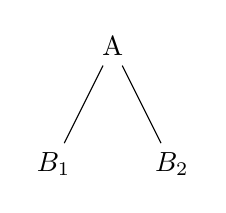
\begin{tikzpicture}
\node {A}
child {node {$B_{1}$}}
child {node {$B_{2}$}
};
\end{tikzpicture}
\end{center}



\subsection{We have Three Conditions for Multi-Valued Dependency}

\begin{itemize}
	\item $A \to B$, for a single value of A, more than one value of B exist .
	\item table should have at least 3 columns .
	\item for this table with $A, B, C$ columns, B and C should be independent .
\end{itemize}







\end{document}